\documentclass[12pt,a4paper]{article}

\usepackage[utf8]{inputenc}
\usepackage[T1]{fontenc}
\usepackage[spanish,es-tabla]{babel}
\usepackage{amsmath}
\usepackage{array}
\usepackage{booktabs}
\usepackage{float}
\usepackage{geometry}
\usepackage{graphicx}
\usepackage{hyperref}
\usepackage{listings}
\usepackage{siunitx}
\usepackage{tabularx}
\usepackage{xcolor}

\geometry{margin=2.7cm}
\emergencystretch=3em
\graphicspath{{../experiments/results/}{assets/}}
\hypersetup{
  colorlinks=true,
  linkcolor=black,
  urlcolor=blue,
  pdftitle={Proyecto 3 - Avance QKD BB84 time-bin},
  pdfauthor={Mateo Sauton e Ignacio Polesello}
}
\sisetup{
  output-decimal-marker={,},
  per-mode=symbol,
  detect-all=true
}
\lstset{
  basicstyle=\ttfamily\small,
  breaklines=true,
  columns=fullflexible,
  frame=single,
  rulecolor=\color{black!25},
  numbers=left,
  numberstyle=\tiny\color{black!50},
  xleftmargin=1.5em,
  framexleftmargin=1.2em
}

\title{
  \textbf{Proyecto 3}\\[0.35em]
  \large Avance del Proyecto Final Integrador\\[0.35em]
  \large Diseño y evaluación por simulación de un banco QKD BB84 en \textit{time-bin}
}
\author{
  Mateo Sauton\\
  Ignacio Polesello\\[0.5em]
  Ingeniería en Telecomunicaciones\\
  Universidad Nacional de San Martín
}
\date{2026}

\begin{document}

\maketitle

\section{Introducción}

Este documento resume el avance del Proyecto Final Integrador orientado al diseño y evaluación por simulación de un banco de pruebas de distribución cuántica de claves (QKD, por sus siglas en inglés) basado en el protocolo BB84 con codificación \textit{time-bin}. El trabajo completo desarrolla el marco teórico, el estado del arte, el análisis de hardware y una propuesta de implementación para un entorno de campus; esta versión, preparada para la materia Proyecto 3, se concentra en cuatro aspectos: introducción, experimentos, resultados y conclusiones.

El problema central que aborda el proyecto es la distribución de claves criptográficas entre dos nodos remotos. En los sistemas actuales, el intercambio de claves suele apoyarse en criptografía de clave pública y en la dificultad computacional de ciertos problemas matemáticos. QKD propone una alternativa complementaria: usar estados cuánticos para detectar la presencia de un observador no autorizado en el canal. Si un atacante intenta medir los estados transmitidos, introduce perturbaciones que se manifiestan como un aumento de la tasa de error cuántico, o QBER (\textit{Quantum Bit Error Rate}). Esa tasa se vuelve una magnitud operativa: si el error es suficientemente bajo, Alice y Bob pueden continuar con tamizado, corrección de errores y amplificación de privacidad; si el error supera el margen admisible, el enlace no debe usarse para extraer una clave secreta.

El protocolo elegido es BB84. En su forma conceptual, Alice prepara bits aleatorios en bases aleatorias y Bob mide cada estado, también con una base elegida al azar. Luego ambos comparan por un canal clásico autenticado qué bases usaron, descartan los eventos con bases incompatibles y conservan una llave tamizada. En una implementación \textit{time-bin}, la información se codifica en la llegada temprana o tardía de pulsos ópticos y en superposiciones entre ambos modos temporales. Esta elección es relevante para fibra óptica porque traduce el problema cuántico a variables propias de telecomunicaciones: pérdidas de canal, sincronización, resolución temporal, visibilidad interferométrica, eficiencia de detección y conteos oscuros.

La hipótesis de trabajo es que un banco QKD de dos nodos puede evaluarse de manera útil mediante simulación antes de construirlo físicamente. La simulación no certifica seguridad criptográfica ni reemplaza una medición experimental, pero sí permite responder preguntas de ingeniería: qué distancia parece razonable, qué tan sensible es el enlace a la eficiencia de detector, cuánto impactan los conteos oscuros, qué visibilidad necesita el interferómetro y cómo cambia la tasa estimada al considerar estados señuelo. Por eso las métricas principales del trabajo son QBER, probabilidad de detección y tasa de llave secreta estimada (SKR, \textit{Secret Key Rate}).

El objetivo general del proyecto es diseñar y evaluar, por simulación y con parámetros realistas, la factibilidad de un enlace QKD BB84 en \textit{time-bin} para dos nodos. Los objetivos específicos son construir el escenario Alice--Bob, ejecutar barridos paramétricos controlados, interpretar los resultados en términos de diseño de hardware y dejar documentadas las limitaciones del modelo. En esta etapa se prioriza una evaluación reproducible y trazable: las corridas se ejecutan desde el repositorio, las figuras se generan desde el script de simulación y las conclusiones se formulan sin asumir que el modelo valida todavía un sistema físico completo.

\section{Experimentos}

Los experimentos se ejecutaron sobre un enlace de dos nodos, Alice y Bob, implementado en SeQUeNCe, un simulador de eventos discretos para redes cuánticas. En este tipo de simulación, el sistema no se calcula como una única fórmula cerrada, sino como una línea temporal de eventos: emisión de pulsos, propagación por el canal, pérdidas, detecciones, mensajes clásicos y finalización de ventanas de protocolo. Este enfoque es adecuado para el proyecto porque permite describir el banco de pruebas con objetos cercanos al lenguaje de telecomunicaciones: nodos, canales, fuente óptica, detector, interferómetro, retardos y métricas.

Alice actúa como nodo emisor. Prepara estados BB84 con codificación \textit{time-bin}, usando una fuente coherente débil con número medio de fotones configurable. Bob actúa como nodo receptor. Mide los estados recibidos con un detector temporal y una rama interferométrica para representar la medición de bases asociadas a superposiciones. Ambos nodos se conectan mediante un canal cuántico de fibra y un canal clásico usado para la coordinación del protocolo.

El procedimiento general fue el mismo para todos los barridos. Primero se definió una variable independiente, por ejemplo distancia o visibilidad. Luego se generó un conjunto de valores para esa variable. Para cada valor se creó una nueva configuración de simulación, se instanciaron Alice, Bob y los canales, se ejecutó BB84 durante un horizonte temporal finito y se registraron las métricas. Finalmente se promediaron los valores obtenidos y se generaron las figuras guardadas en \texttt{experiments/results/}.

\begin{table}[H]
  \centering
  \begin{tabularx}{\textwidth}{p{0.27\textwidth}p{0.22\textwidth}X}
    \toprule
    Parámetro & Valor base & Interpretación \\
    \midrule
    Atenuación de fibra & \SI{0.2}{\decibel\per\kilo\meter} & Pérdida típica usada para modelar propagación óptica. \\
    Frecuencia de fuente & \SI{80}{\mega\hertz} & Tasa de repetición elegida para mantener corridas computacionalmente manejables. \\
    Longitud de llave & 128 bits & Tamaño de muestra de simulación; no representa una llave final de producción. \\
    Número medio de fotones & 0,1 o barrido & Intensidad de fuente coherente débil. \\
    Eficiencia de detector & 0,1 o barrido & Probabilidad efectiva de detectar un fotón incidente. \\
    Conteos oscuros & \SI{100}{\hertz} o barrido & Clicks del detector no asociados a fotones de la señal. \\
    Visibilidad & 0,98 o barrido & Calidad de interferencia del receptor \textit{time-bin}. \\
    Resolución temporal & \SI{10}{\pico\second} & Capacidad del detector para distinguir ventanas temporales. \\
    \bottomrule
  \end{tabularx}
  \caption{Parámetros base usados en las simulaciones.}
  \label{tab:p3_parametros}
\end{table}

El siguiente fragmento resume la clase de parámetros usada por el script. Su función es concentrar en una sola estructura las variables físicas y protocolarias que se modifican en cada experimento. Esto permite cambiar una variable por vez y mantener constante el resto del sistema, condición necesaria para interpretar correctamente cada curva.

\begin{lstlisting}[language=Python, caption={Estructura de parámetros usada para crear cada punto de simulación.}]
@dataclass
class SimParams:
    distance_km: float
    attenuation_db_km: float = DEFAULT_ALPHA_DB_KM
    detector_efficiency: float = 0.1
    dark_count_hz: float = 100.0
    mean_photon_num: float = 0.1
    frequency_hz: float = DEFAULT_FREQUENCY_HZ
    visibility: float = 0.98
    key_length: int = DEFAULT_KEY_LENGTH
    num_keys: int = DEFAULT_NUM_KEYS
    runtime_ps: float = DEFAULT_RUNTIME_PS
\end{lstlisting}

La topología del enlace se construye creando una línea temporal, un canal cuántico, un canal clásico y dos nodos QKD. La distancia aparece dentro de los canales, no como un dato externo aislado; por lo tanto, modificar la distancia cambia las pérdidas y retardos asociados a la propagación. Esta estructura es la que permite que los barridos de distancia, detector y visibilidad usen el mismo modelo base.

\begin{lstlisting}[language=Python, caption={Creación simplificada del enlace Alice--Bob.}]
tl = Timeline(p.runtime_ps)

qc0 = QuantumChannel("qc0", tl, distance=distance_m,
                     attenuation=attenuation_db_m,
                     frequency=p.frequency_hz)
cc0 = ClassicalChannel("cc0", tl, distance=distance_m)

alice = QKDNode("alice", tl, encoding=time_bin, stack_size=1)
bob = QKDNode("bob", tl, encoding=time_bin, stack_size=1)
\end{lstlisting}

También se parametriza el receptor. La eficiencia y los conteos oscuros se aplican a los detectores de Bob. La visibilidad del interferómetro se traduce a un error de fase con la relación \(p_\text{fase}=(1-V)/2\). Esta traducción es importante porque convierte una magnitud óptica, la calidad de interferencia, en una fuente de error que afecta QBER.

\begin{lstlisting}[language=Python, caption={Mapeo de parámetros del receptor al modelo simulado.}]
phase_error = max(0.0, min(1.0, (1.0 - p.visibility) / 2.0))
qsd = bob.components["bob.qsdetector"]

for i in range(3):
    bob.update_detector_params(i, "efficiency", p.detector_efficiency)
    bob.update_detector_params(i, "dark_count", p.dark_count_hz)
    bob.update_detector_params(i, "time_resolution", p.time_resolution_ps)

qsd.update_interferometer_params("phase_error", phase_error)
\end{lstlisting}

\subsection*{Experimento 1: distancia de fibra}

El primer experimento buscó estimar cómo se degrada el enlace al aumentar la longitud de fibra. La pregunta técnica fue: ¿hasta qué distancia el enlace simulado conserva una QBER suficientemente baja y una SKR no nula? Para responderla, se barrió la distancia entre valores cortos y largos, manteniendo constantes la eficiencia de detector, los conteos oscuros, la intensidad de fuente y la visibilidad.

Lo esperado era una caída de la probabilidad de detección al aumentar la distancia, porque la transmitancia de una fibra con atenuación expresada en dB/km disminuye exponencialmente con la longitud. También se esperaba que la SKR disminuyera, ya que una menor cantidad de eventos detectados reduce la cantidad de bits útiles por unidad de tiempo. El QBER podía mantenerse bajo en distancias moderadas y crecer en zonas de baja señal, donde el enlace se vuelve más sensible al ruido y a la dispersión estadística.

Este barrido aporta una primera decisión de diseño: define rangos de distancia razonables para comenzar una prueba de laboratorio o campus. Si el enlace no acumula detecciones suficientes o supera el umbral de QBER, no conviene usar esa distancia como condición inicial de calibración.

\subsection*{Experimento 2: sensibilidad del detector}

El segundo experimento estudió el impacto de dos parámetros del receptor: eficiencia de detección y conteos oscuros. La distancia se fijó en \SI{50}{\kilo\meter}. En una primera parte se barrió la eficiencia del detector, manteniendo constantes los conteos oscuros. En una segunda parte se barrió la tasa de conteos oscuros, manteniendo fija la eficiencia.

La expectativa era que una mayor eficiencia aumentara la cantidad de eventos útiles y favoreciera la SKR, siempre que el QBER se mantuviera bajo. En cambio, un aumento de conteos oscuros debía elevar la probabilidad de clicks no correlacionados con el estado enviado. Esos clicks pueden introducir errores, especialmente cuando la señal recibida es débil.

Este experimento es relevante porque el detector es uno de los componentes más críticos de un banco QKD. En una implementación real no alcanza con elegir cualquier detector óptico: hay que considerar eficiencia cuántica, dark count rate, dead time, jitter, resolución temporal y compatibilidad con la tasa de repetición. El barrido permite ver cuáles de estas variables tienen mayor impacto dentro del modelo usado.

\subsection*{Experimento 3: visibilidad interferométrica}

El tercer experimento analizó la visibilidad del interferómetro. En codificación \textit{time-bin}, Bob no solo debe distinguir pulsos tempranos y tardíos; también debe medir superposiciones entre ambos modos temporales. Para eso se requiere interferencia estable. Si la visibilidad es baja, la medición de fase se degrada y aumenta la probabilidad de error.

Se fijó la distancia en \SI{30}{\kilo\meter} y se barrió la visibilidad entre valores moderados y cercanos a uno. Para cada punto, el script convirtió la visibilidad en error de fase y ejecutó el mismo protocolo BB84. Se esperaba que visibilidades altas produjeran menor QBER y mayor SKR, mientras que visibilidades bajas redujeran el rendimiento del enlace aunque la distancia no fuera extrema.

Este experimento conecta directamente el modelo con una exigencia de hardware. La visibilidad depende de balance de caminos, estabilidad térmica, alineación, polarización y control mecánico. Por lo tanto, la simulación muestra que el interferómetro no es un detalle secundario del receptor, sino una pieza central para que BB84 \textit{time-bin} funcione con baja tasa de error.

\subsection*{Experimento 4: comparación con estados señuelo}

El cuarto experimento comparó una estimación simple de SKR con una estimación que incorpora estados señuelo de forma analítica. La motivación es que una fuente coherente débil no emite siempre un único fotón: su número de fotones por pulso sigue una distribución de Poisson. Algunos pulsos pueden contener más de un fotón, lo que abre riesgos de seguridad frente a ataques que explotan eventos multifotónicos. Los estados señuelo permiten estimar mejor la contribución segura de los eventos monofotónicos.

En la simulación se compararon dos curvas entre distancias de \SI{5}{\kilo\meter} y \SI{90}{\kilo\meter}. La primera curva usa una tasa simple calculada a partir de QBER y throughput simulados. La segunda combina errores simulados con cotas analíticas decoy usando una intensidad de señal \(\mu=0,6\), una intensidad señuelo \(\nu=0,2\) y una intensidad de vacío efectiva pequeña.

La expectativa era que ambas tasas disminuyeran con la distancia y que la cota decoy quedara por debajo de la estimación simple. Esta diferencia no significa que los estados señuelo empeoren el enlace, sino que la estimación decoy es más conservadora y más cercana a una interpretación de seguridad realista para fuentes coherentes débiles. En esta etapa, el experimento decoy debe leerse como una comparación conceptual y de diseño, no como una implementación protocolar completa de decoy states dentro de SeQUeNCe.

\section{Resultados de los experimentos}

La Figura~\ref{fig:p3_exp1_distance} muestra el resultado del barrido de distancia. La probabilidad de detección cae de forma sostenida al aumentar la longitud de fibra, comportamiento consistente con el presupuesto de pérdidas. El QBER se mantiene bajo en buena parte del barrido y aumenta con fuerza hacia el extremo superior, donde la señal útil se vuelve más escasa y la corrida queda más expuesta a ruido y fluctuaciones estadísticas.

\begin{figure}[H]
  \centering
  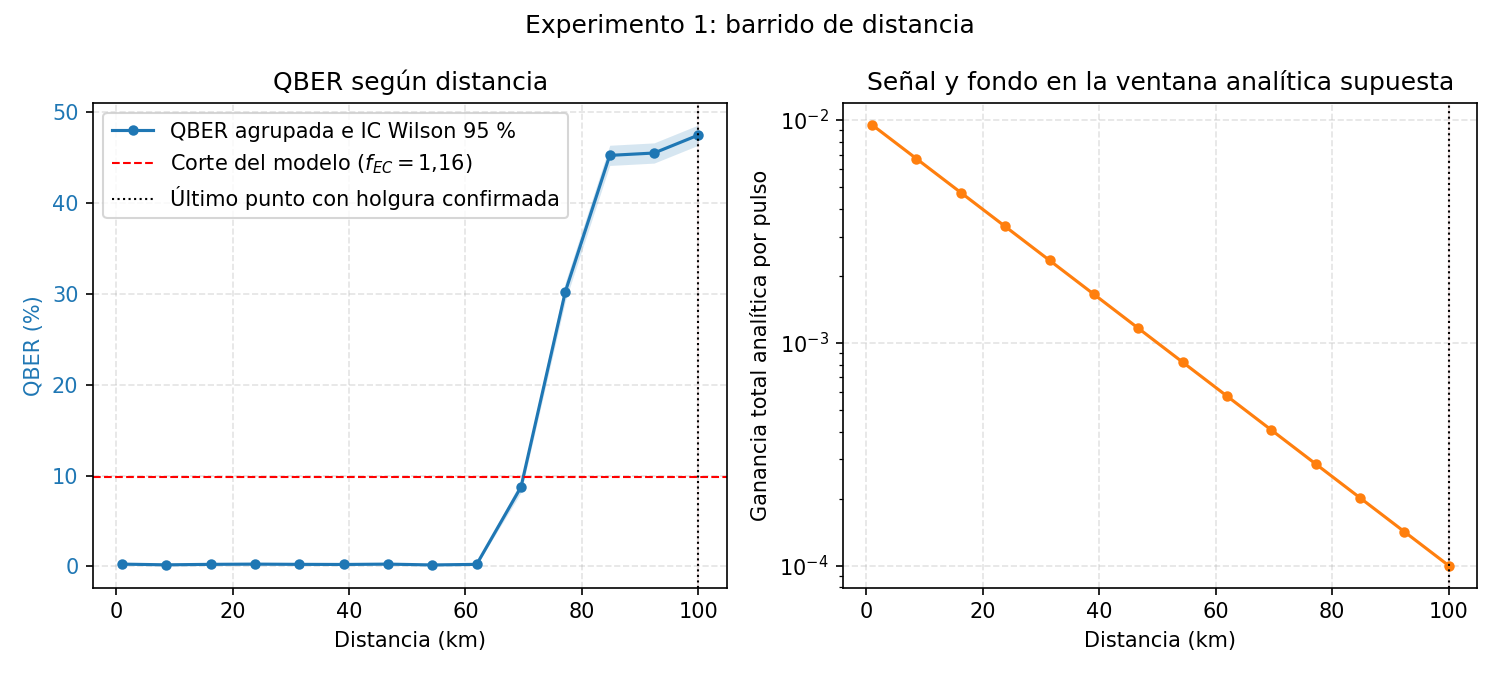
\includegraphics[width=\textwidth]{exp1_distance_sweep.png}
  \caption{QBER y probabilidad de detección en función de la distancia de fibra.}
  \label{fig:p3_exp1_distance}
\end{figure}

La Figura~\ref{fig:p3_exp1_skr} presenta la SKR estimada para el mismo barrido. La tasa disminuye con la distancia y se anula cuando el QBER supera el umbral de referencia usado por el modelo. La lectura de ingeniería es directa: distancias cortas y moderadas son más apropiadas para validar el banco, mientras que distancias largas exigen mayor control de pérdidas, ruido y estabilidad.

\begin{figure}[H]
  \centering
  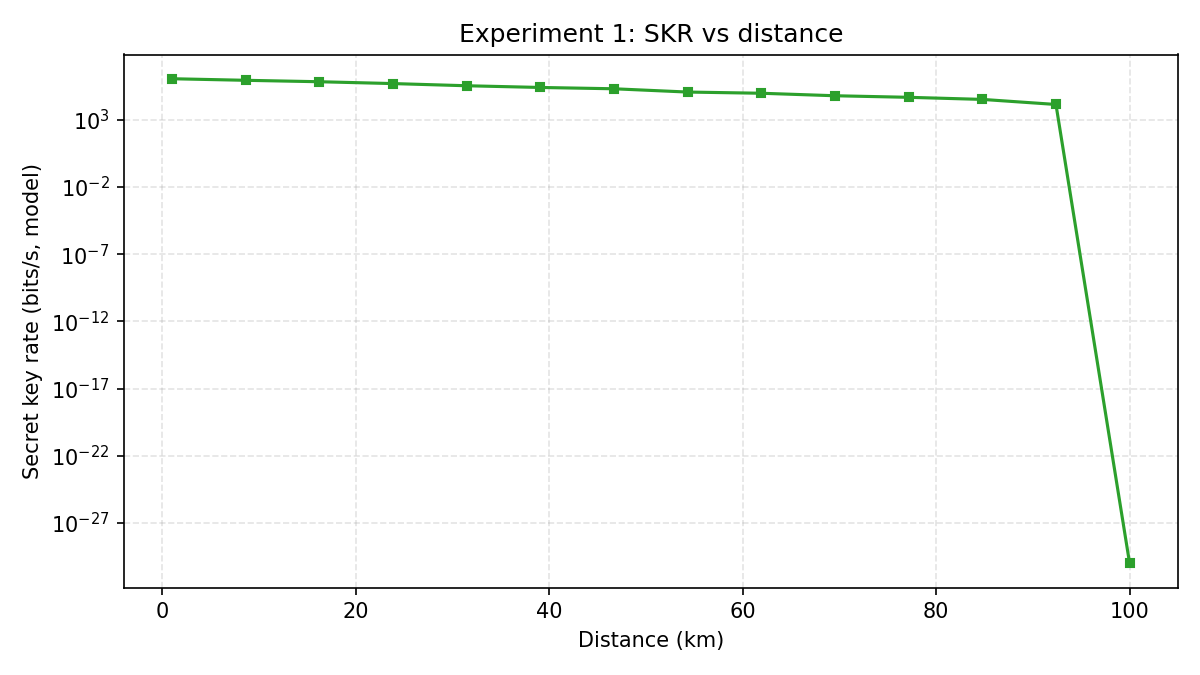
\includegraphics[width=0.92\textwidth]{exp1_skr_distance.png}
  \caption{Tasa de llave secreta estimada en función de la distancia.}
  \label{fig:p3_exp1_skr}
\end{figure}

La Figura~\ref{fig:p3_exp2_detector} resume el experimento de sensibilidad del detector. En el barrido de eficiencia, el QBER permanece por debajo del umbral en los puntos simulados y la SKR muestra cambios asociados a la eficiencia y al tamaño finito de muestra. En el barrido de conteos oscuros, el error no domina fuertemente bajo los parámetros elegidos. Esto sugiere que, en esta configuración, la acumulación de eventos útiles y la eficiencia efectiva del receptor tienen un rol más visible que los dark counts dentro del rango evaluado.

\begin{figure}[H]
  \centering
  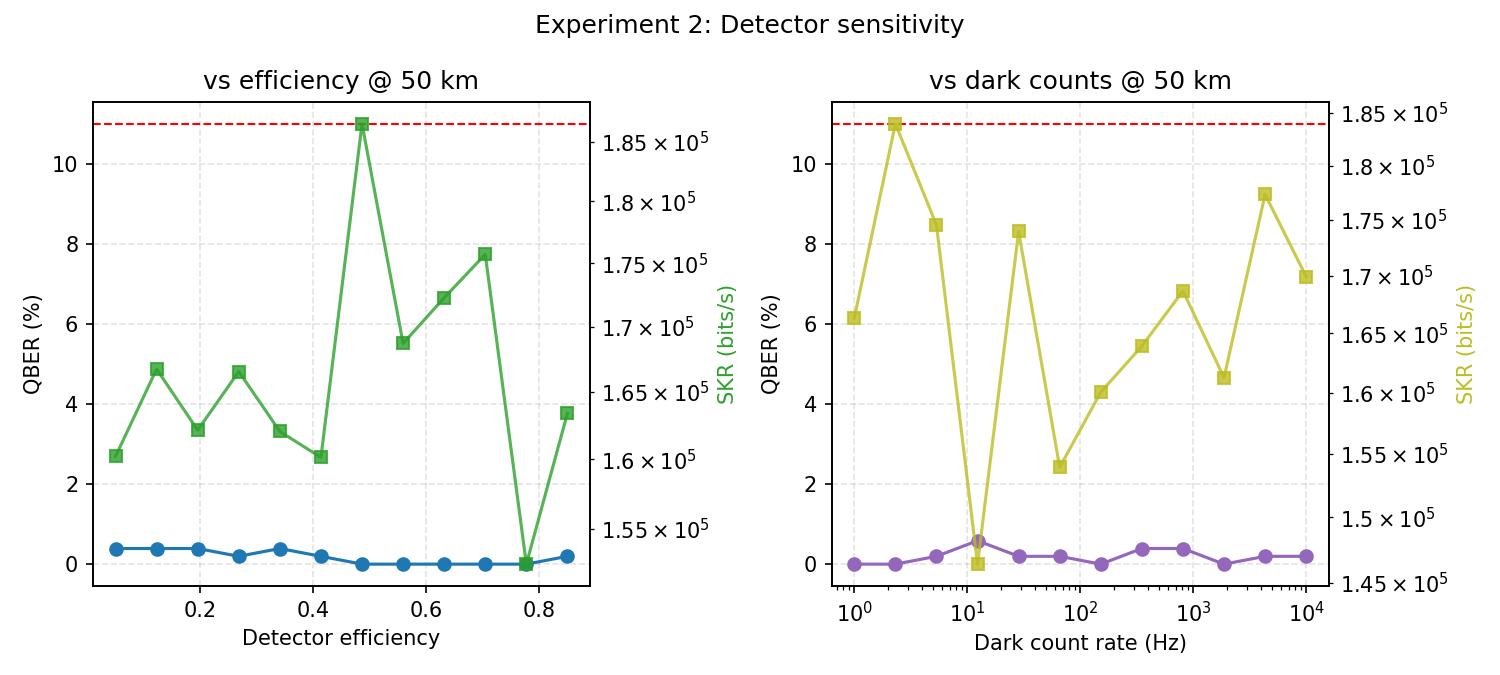
\includegraphics[width=\textwidth]{exp2_detector_sensitivity.png}
  \caption{QBER y SKR frente a eficiencia de detector y conteos oscuros a distancia fija.}
  \label{fig:p3_exp2_detector}
\end{figure}

La Figura~\ref{fig:p3_exp3_visibility} muestra el barrido de visibilidad. La tendencia esperada se observa en el comportamiento general: visibilidades más altas favorecen QBER más bajo y tasas secretas más altas. La curva no es perfectamente monótona porque cada punto se obtiene con llaves cortas y un número limitado de repeticiones, pero la conclusión de diseño se mantiene: la estabilidad interferométrica es crítica en una implementación \textit{time-bin}.

\begin{figure}[H]
  \centering
  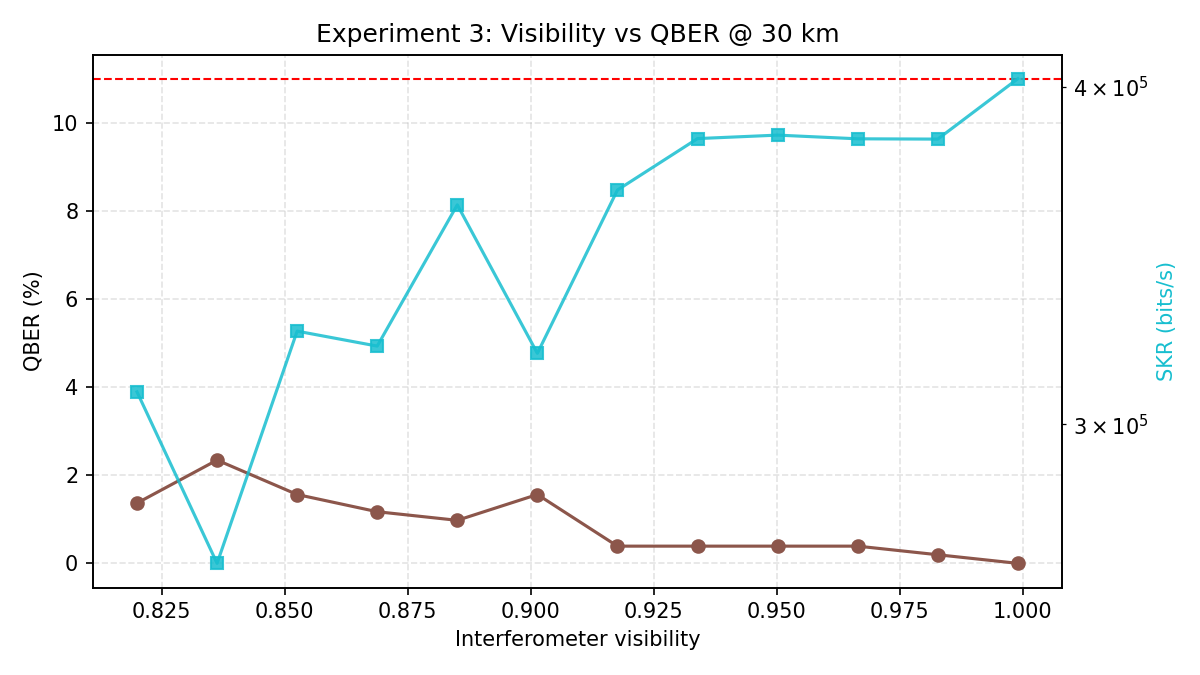
\includegraphics[width=0.92\textwidth]{exp3_visibility.png}
  \caption{QBER y SKR en función de la visibilidad del interferómetro.}
  \label{fig:p3_exp3_visibility}
\end{figure}

La Figura~\ref{fig:p3_exp4_decoy} compara la estimación sin estados señuelo con la cota decoy. Ambas curvas disminuyen con la distancia. La curva decoy queda por debajo de la estimación simple porque intenta acotar la contribución segura de eventos monofotónicos en presencia de una fuente coherente débil. Por lo tanto, el resultado no debe interpretarse como una pérdida causada por usar señuelos, sino como una estimación más conservadora de la tasa que podría defenderse bajo supuestos de seguridad más realistas.

\begin{figure}[H]
  \centering
  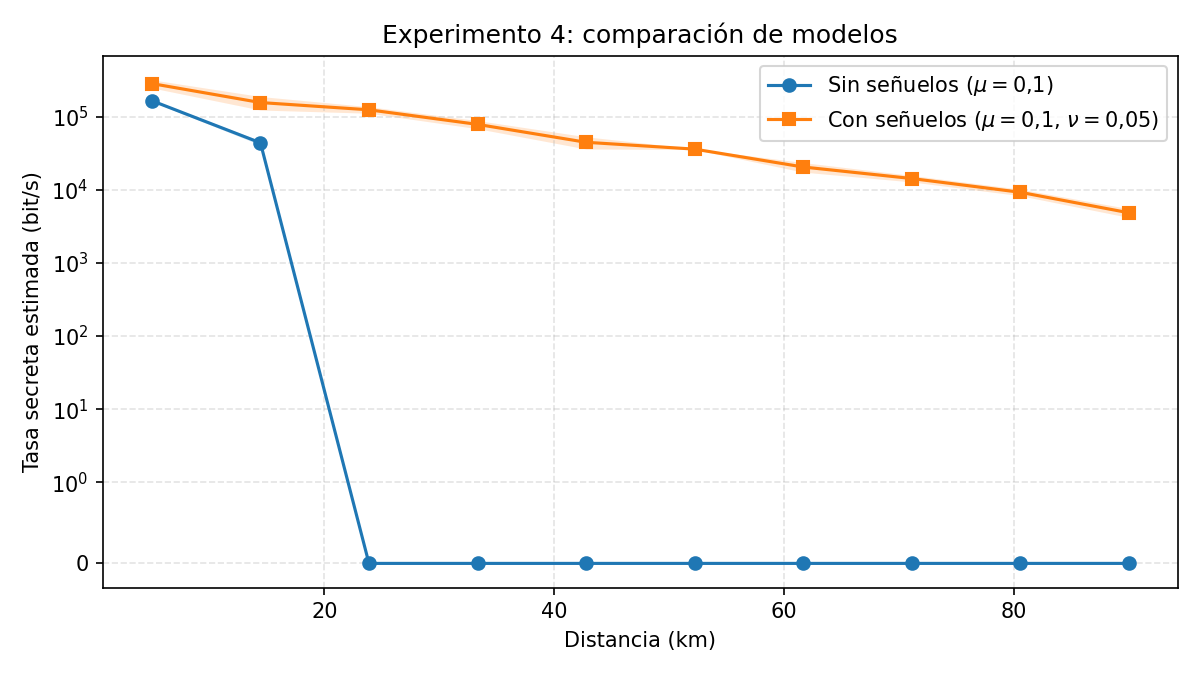
\includegraphics[width=0.92\textwidth]{exp4_decoy_impact.png}
  \caption{Comparación de SKR estimada sin estados señuelo y con cota analítica decoy.}
  \label{fig:p3_exp4_decoy}
\end{figure}

\begin{table}[H]
  \centering
  \begin{tabularx}{\textwidth}{p{0.25\textwidth}X}
    \toprule
    Experimento & Resultado principal \\
    \midrule
    Distancia & La atenuación reduce la probabilidad de detección y termina degradando la SKR al aumentar la longitud de fibra. \\
    Detector & La eficiencia de detección afecta la tasa útil; los conteos oscuros no dominan el error en el rango evaluado. \\
    Visibilidad & La calidad interferométrica es una variable crítica para mantener QBER bajo en \textit{time-bin}. \\
    Estados señuelo & La cota decoy entrega una tasa más conservadora y conceptualmente más adecuada para fuentes coherentes débiles. \\
    \bottomrule
  \end{tabularx}
  \caption{Síntesis de resultados de diseño.}
  \label{tab:p3_sintesis}
\end{table}

En conjunto, los resultados muestran que la simulación cumple su función como herramienta de avance del proyecto. No entrega una especificación final cerrada del banco físico, pero sí identifica las variables dominantes: pérdida de fibra, eficiencia de detección, visibilidad interferométrica y modelo de seguridad asociado a la fuente óptica.

\section{Conclusiones}

El avance presentado permite sostener que la simulación de un enlace QKD BB84 en \textit{time-bin} es una herramienta útil para diseñar un banco de pruebas antes de su implementación física. El modelo de dos nodos permite estudiar cómo cambian QBER, probabilidad de detección y SKR frente a variables de ingeniería concretas. Esto aporta una base para decidir qué condiciones conviene ensayar primero y qué componentes requieren mayor atención.

El barrido de distancia confirma el rol dominante de la atenuación de fibra. A mayor longitud, menor probabilidad de detección y menor tasa estimada. Para una futura prueba física, esto sugiere comenzar por un enlace corto o moderado, validar sincronización y detección, y recién después avanzar hacia distancias mayores. El barrido de detector muestra que la eficiencia es una variable relevante para acumular eventos útiles, mientras que los conteos oscuros, en el rango simulado, no son la fuente dominante de error. Aun así, en hardware real deben medirse junto con jitter, dead time y ventanas temporales.

El barrido de visibilidad confirma que la calidad interferométrica es central para una codificación \textit{time-bin}. Un receptor puede tener buena eficiencia y aun así producir una QBER elevada si la interferencia no es estable. Esto vuelve prioritario el diseño óptico del receptor: balance de caminos, estabilidad térmica, control de polarización y resolución temporal deben tratarse como requisitos de primer orden.

La comparación con estados señuelo muestra una diferencia conceptual importante entre rendimiento observable y tasa segura estimada. Una curva simple de SKR puede servir para evaluar desempeño, pero no alcanza para discutir seguridad práctica con fuentes coherentes débiles. La estimación decoy es más conservadora porque intenta aislar la contribución segura de los eventos monofotónicos. En esta etapa, el resultado decoy funciona como una primera aproximación analítica; una versión futura debería implementar el protocolo decoy completo dentro del flujo de simulación.

Como conclusión general, el proyecto avanzó desde una idea amplia de red QKD hacia un experimento reproducible con métricas y figuras concretas. Para la entrega de Proyecto 3, el aporte principal es mostrar que ya existe un modelo funcional, que se ejecutaron barridos relevantes y que los resultados permiten orientar decisiones de diseño. Para la tesis completa, los pasos siguientes son profundizar la validación estadística, ampliar la conexión con hardware real, relevar condiciones de implementación en campus y documentar con mayor detalle las limitaciones de seguridad y postprocesamiento.

\end{document}
